\documentclass{beamer}[10]

\usepackage{graphicx}
\usepackage{xcolor}
\usepackage{tabto}
%\usepackage{beamerthemesplit}
\usepackage{tikz}
\usepackage{cancel}
\usepackage{verbatim}
\usepackage{fancybox}
\usepackage{enumerate}
\usepackage{amsmath,amssymb,amsthm,textcomp,mathtools}
\usepackage[super]{nth}
\usepackage[amssymb]{SIunits}
\usepackage{booktabs}
\usepackage{cancel}
\usepackage{bm}
\usepackage[utf8]{inputenc}
\usepackage{tabularx}
\usepackage{ragged2e}
\newcolumntype{Y}{ >{\RaggedRight\arraybackslash}X}
\usetikzlibrary{arrows,shapes}
\newcommand\T{\rule{0pt}{2.6ex}}
\newcommand\B{\rule[-1.2ex]{0pt}{0pt}}
\definecolor{UUcrimson}{RGB}{204,0,0}
\mode<presentation>
{ \usetheme{default}
  \usecolortheme[named=UUcrimson]{structure}
  \useinnertheme{circles}
  \setbeamercovered{transparent}
  \setbeamertemplate{blocks}[rounded]
  \usefonttheme[onlymath]{serif}
  \setbeamertemplate{navigation symbols}{}
  \setbeamertemplate{footline}[page number]
  \setbeamertemplate{navigation symbols}{}
  \setbeamercolor{section in toc}{fg=black,bg=white}
  \setbeamercolor{alerted text}{fg=UUcrimson!80!gray}
  \setbeamercolor*{palette primary}{fg=white,bg=UUcrimson}
  \setbeamercolor*{palette secondary}{fg=UUcrimson!70!black,bg=gray!15!white}
  \setbeamercolor*{palette tertiary}{bg=UUcrimson!80!black,fg=gray!10!white}
  \setbeamercolor*{palette quaternary}{fg=UUcrimson,bg=gray!5!white}
  \setbeamercolor*{palette sidebar primary}{fg=UUcrimson!10!black}
  \setbeamercolor*{palette sidebar secondary}{fg=white}
  \setbeamercolor*{palette sidebar tertiary}{fg=UUcrimson!50!black}
  \setbeamercolor*{palette sidebar quaternary}{fg=gray!10!white}
  \setbeamercolor{titlelike}{parent=palette primary,fg=white}
  \setbeamercolor{frametitle}{bg=UUcrimson}
  \setbeamercolor{frametitle right}{bg=UUcrimson}
  \setbeamercolor*{separation line}{}
  \setbeamercolor*{fine separation line}{}
}

\usetikzlibrary{backgrounds}
\makeatletter
\tikzstyle{every picture}+=[remember picture]
\tikzset{%
  fancy quotes/.style={
    text width=\fq@width pt,
    align=justify,
    inner sep=1em,
    anchor=north west,
    minimum width=\linewidth,
    font=\itshape
  },
  fancy quotes width/.initial={.8\linewidth},
  fancy quotes marks/.style={
    scale=8,
    text=white,
    inner sep=0pt,
  },
  fancy quotes opening/.style={
    fancy quotes marks,
  },
  fancy quotes closing/.style={
    fancy quotes marks,
  },
  fancy quotes background/.style={
    show background rectangle,
    inner frame xsep=0pt,
    background rectangle/.style={
      fill=gray!25,
      rounded corners,
    },
  }
}
\newenvironment{fancyquotes}[1][]{%
\noindent
\tikzpicture[fancy quotes background]
\node[fancy quotes opening,anchor=north west] (fq@ul) at (0,0) {``};
\tikz@scan@one@point\pgfutil@firstofone(fq@ul.east)
\pgfmathsetmacro{\fq@width}{\linewidth - 2*\pgf@x}
\node[fancy quotes,#1] (fq@txt) at (fq@ul.north west) \bgroup}
{\egroup;
\node[overlay,fancy quotes closing,anchor=east] at (fq@txt.south east) {''};
\endtikzpicture}
\makeatother


\usetikzlibrary{backgrounds}
\makeatletter
\tikzstyle{every picture}+=[remember picture]
\tikzset{%
  fancy defs/.style={
    text width=\fq@width pt,
    align=justify,
    inner sep=0.25em,
    anchor=north west,
    minimum width=\linewidth,
    font=\itshape
  },
  fancy defs width/.initial={.8\linewidth},
  fancy defs marks/.style={
    scale=8,
    text=white,
    inner sep=0pt,
  },
  fancy defs opening/.style={
    fancy defs marks,
  },
  fancy defs closing/.style={
    fancy defs marks,
  },
  fancy defs background/.style={
    show background rectangle,
    inner frame xsep=0pt,
    background rectangle/.style={
      fill=gray!25,
      rounded corners,
    },
  }
}
\newenvironment{fancydefs}[1][]{%
\noindent
\tikzpicture[fancy defs background]
\node[fancy defs opening,anchor=north west] (fq@ul) at (0,0) {};
\tikz@scan@one@point\pgfutil@firstofone(fq@ul.east)
\pgfmathsetmacro{\fq@width}{\linewidth - 2*\pgf@x}
\node[fancy defs,#1] (fq@txt) at (fq@ul.north west) \bgroup}
{\egroup;
\node[overlay,fancy defs closing,anchor=east] at (fq@txt.south east) {};
\endtikzpicture}
\makeatother
\usepackage{scalerel}[2014/03/10]
\usepackage{stackengine}
\usepackage{empheq}
\newcommand*\widefbox[1]{\fbox{\hspace{0.5em}#1\hspace{0.5em}}}

\newcommand\reallywidetilde[1]{\ThisStyle{%
  \setbox0=\hbox{$\SavedStyle#1$}%
  \stackengine{-.1\LMpt}{$\SavedStyle#1$}{%
    \stretchto{\scaleto{\SavedStyle\mkern.2mu\sim}{.5467\wd0}}{.4\ht0}%
%    .2mu is the kern imbalance when clipping white space
%    .5467++++ is \ht/[kerned \wd] aspect ratio for \sim glyph
  }{O}{c}{F}{T}{S}%
}}
\usepackage{media9}

\logo{
\includegraphics[width=0.75cm]{logo.jpg}}
\author[Gibbs]{Dr. Jeremy A. Gibbs}
\institute{Department of Mechanical Engineering\\University of Utah}
\date{Spring 2017}
\title{Environmental Fluid Dynamics: Lecture 18}
% colors
\newcommand{\ihat}{\boldsymbol{\hat{\imath}}}
\newcommand{\jhat}{\boldsymbol{\hat{\jmath}}}
\newcommand{\khat}{\boldsymbol{\hat{k}}}
\definecolor{colororange}{HTML}{E65100} % orange
\definecolor{colordgray}{HTML}{795548} % dark gray for note
\definecolor{colorhgray}{HTML}{212121} % heavy dark gray for normal text
\definecolor{colorgreen}{HTML}{009688} % green
\definecolor{colorwhite}{HTML}{FFFFFF} % background white
\definecolor{colorlgray}{HTML}{F5F3EE} % background light gray
\definecolor{colorblue}{HTML}{0277BB} % blue
\definecolor{colorred}{HTML}{CC0000} % red
\newcommand{\fontsizeone}{1.9em}
\setbeamertemplate{caption}{\raggedright\insertcaption\par}
\newcommand{\framecard}[2][colorgreen]{
  {\setbeamercolor{background canvas}{bg=#1}
    \begin{frame}[plain]
    \vfill
    \begin{center}
     {#2}
    \end{center}
    \vfill
    \end{frame}
  }
}
\settowidth{\leftmargini}{\usebeamertemplate{itemize item}}
\addtolength{\leftmargini}{\labelsep}
\usepackage{empheq}
\begin{document}

%----------------------------------------------------------------------------------------
%	TITLE & TOC SLIDES
%----------------------------------------------------------------------------------------

\begin{frame} 
  \titlepage
\end{frame}

%------------------------------------------------

\begin{frame}
\frametitle{Overview}
\tableofcontents
\end{frame}

%------------------------------------------------
\section{Turbulence Kinetic Energy Balance}     %
%------------------------------------------------
\framecard[colorred]{{\color{white}\Huge\begin{center}Turbulence Kinetic~\\Energy Balance\end{center}}}
%------------------------------------------------
\begin{frame}{Turbulence Kinetic Energy Balance}
\begin{itemize}
  	\item We previously derived the following generic expression for turbulent momentum flux.
  	\begin{align*}
  	\frac{\partial (\overline{u_k^\prime u_i^\prime})}{\partial t} &= - \overline u_j \frac{\partial (\overline{u_k^\prime u_i^\prime})}{\partial x_j} - \left[\overline{u_j^\prime u_i^\prime}\frac{\partial \overline u_k}{\partial x_j} + \overline{u_k^\prime u_j^\prime}\frac{\partial \overline u_i}{\partial x_j}\right] - \frac{\partial (\overline{u_k^\prime u_j^\prime u_i^\prime})}{\partial x_j} \\&\hphantom{=\ }+ \overline{u_k^\prime b^\prime}\delta_{i3} + \overline{u_i^\prime b^\prime}\delta_{k3}\\&\hphantom{=\ }-\left[ \frac{\partial(\overline{u_k^\prime \Pi^\prime})}{\partial x_i} + \frac{\partial(\overline{u_i^\prime \Pi^\prime})}{\partial x_k}\right. - \left.\overline{\Pi^\prime \left(\frac{\partial u_k^\prime}{\partial x_i} + \frac{\partial u_i^\prime}{\partial x_k}\right)}\right] \\&\hphantom{=\ }+\nu \frac{\partial^2 (\overline{u_k^\prime u_i^\prime})}{\partial x_j^2} - 2\nu \overline{\frac{\partial u_k^\prime}{\partial x_j}\frac{\partial u_i^\prime}{\partial x_j}}
  	\end{align*}
  	\item We will manipulate this equation to derive the turbulence kinetic energy (TKE) balance equation
  \end{itemize}
\end{frame}
%------------------------------------------------
\begin{frame}{Turbulence Kinetic Energy Balance}
\textbf{A pedantic aside}
\begin{itemize}
  	\item You might often see TKE written as \textit{turbulent} kinetic energy. 
  	\item No! Stop that!
  	\item Writing turbulent kinetic energy implies that there is some kinetic energy that is itself turbulent.
  	\item The more accurate name is \textit{turbulence} kinetic energy.
  	\item Here, we describe kinetic energy that arises due to eddies in a turbulent flow.
  \end{itemize}
\end{frame}
%------------------------------------------------
\begin{frame}{Turbulence Kinetic Energy Balance}
\begin{itemize}
  	\item We want an expression for TKE ($\overline{e}=0.5\overline{u_i^\prime u_i^\prime}$).
  	\item So, we set $k=i$ and divide by 2:
  	\begin{align*}
  	\frac{1}{2}\frac{\partial (\overline{u_i^\prime u_i^\prime})}{\partial t} &= - \frac{1}{2}\overline u_j \frac{\partial (\overline{u_i^\prime u_i^\prime})}{\partial x_j} -\frac{1}{2} \left[\overline{u_j^\prime u_i^\prime}\frac{\partial \overline u_i}{\partial x_j} + \overline{u_i^\prime u_j^\prime}\frac{\partial \overline u_i}{\partial x_j}\right] - \frac{1}{2}\frac{\partial (\overline{u_i^\prime u_j^\prime u_i^\prime})}{\partial x_j} \\&\hphantom{=\ }+\frac{1}{2} \overline{u_i^\prime b^\prime}\delta_{i3} + \frac{1}{2}\overline{u_i^\prime b^\prime}\delta_{k3}\\&\hphantom{=\ }-\frac{1}{2}\left[ \frac{\partial(\overline{u_i^\prime \Pi^\prime})}{\partial x_i} + \frac{\partial(\overline{u_i^\prime \Pi^\prime})}{\partial x_i}\right. - \left.\overline{\Pi^\prime \left(\frac{\partial u_i^\prime}{\partial x_i} + \frac{\partial u_i^\prime}{\partial x_i}\right)}\right] \\&\hphantom{=\ }+\frac{1}{2}\nu \frac{\partial^2 (\overline{u_i^\prime u_i^\prime})}{\partial x_j^2} - \frac{1}{2}2\nu \overline{\frac{\partial u_i^\prime}{\partial x_j}\frac{\partial u_i^\prime}{\partial x_j}}
  	\end{align*}
  \end{itemize}
\end{frame}
%------------------------------------------------
\begin{frame}{Turbulence Kinetic Energy Balance}
\begin{itemize}
  	\item Substituting $\overline{e}=0.5\overline{u_i^\prime u_i^\prime}$ and simplifying yields
  	\begin{empheq}[box=\widefbox]{align}
  	\label{eq1}
\underbrace{\vphantom{\overline u_j \frac{\partial \overline e}{\partial x_j}}\frac{\partial \overline{e}}{\partial t}}_{1} =&- \underbrace{\overline u_j \frac{\partial \overline e}{\partial x_j}}_{2} -\underbrace{\overline{u_j^\prime u_i^\prime}\frac{\partial \overline u_i}{\partial x_j}}_{3} - \underbrace{\frac{\partial (\overline{u_j^\prime e})}{\partial x_j}}_{4} + \underbrace{\vphantom{\overline u_j \frac{\partial \overline e}{\partial x_j}}\overline{u_i^\prime b^\prime}\delta_{i3}}_{5} \\&- \underbrace{\frac{\partial (\overline{u_i^\prime \Pi^\prime})}{\partial x_i}}_{6} +\underbrace{\nu \frac{\partial^2 \overline{e}}{\partial x_j^2}}_{7}-\underbrace{\nu \overline{\frac{\partial u_i^\prime}{\partial x_j}\frac{\partial u_i^\prime}{\partial x_j}}}_{8}\nonumber
\end{empheq}
  \end{itemize}
\end{frame}
%------------------------------------------------
\begin{frame}{Turbulence Kinetic Energy Balance}
\textbf{\underline{Terms in Eq.~(\ref{eq1})}}
\begin{enumerate}
	\item Storage of tke
	\item Advection of tke by the mean wind
	\item Production of tke by the mean wind shear
	\item Transport of tke by turbulent motions (turbulent diffusion)
	\item Production/destruction of tke by buoyancy
	\item Transport of tke by pressure (pressure diffusion)
	\item Molecular diffusion of tke
	\item Viscous dissipation of tke
\end{enumerate}
\end{frame}
%------------------------------------------------
\begin{frame}{Turbulence Kinetic Energy Balance}
\textbf{Term 1}
\begin{itemize}
	\item $\partial \overline{e}/\partial t$ is very small at night, $\sim 2\ \metre\squared\; \second\rpsquared$ during the day in the surface layer, and is often neglected over oceans.
\end{itemize}
~\\~\\
\textbf{Term 2}
\begin{itemize}
	\item Advection can vary widely, but is usually considered negligible over large areas ($10\ \kilo\metre \times 10\ \kilo\metre$).
	\item The term becomes important over smaller areas, where heterogeneity matters.
\end{itemize}
\end{frame}
%------------------------------------------------
\begin{frame}{Turbulence Kinetic Energy Balance}
\textbf{Term 3}
\begin{itemize}
	\item Shear production describes the interaction between the flux and gradient.
	\item The effect is strongest at the surface.
\end{itemize}
~\\~\\
\textbf{Term 4}
\begin{itemize}
	\item Turbulent transport is advection by velocity fluctuations.
	\item This is not a source term because it integrates to zero over the entire domain (i.e., it redistributes TKE)
\end{itemize}
\end{frame}
%------------------------------------------------
\begin{frame}{Turbulence Kinetic Energy Balance}
\textbf{Term 5}
\begin{itemize}
	\item Buoyancy generally maxes at during the daytime hours at $\sim 0.25\ \kelvin\ \metre\reciprocal\second$
	\item Buoyancy is especially important during the day because it affects thermals.
	\item We can define the Deardorff scaling velocity for the mixed layer using vertical buoyancy flux.
	$$w_* = (\overline{w^\prime b^\prime})^{1/3}$$
	\item For $b>0$ (unstable), an air parcel displaced by turbulence continues to move in the direction of the displacement. Thus, there is production of 
	\item For $b<0$ (stable), an air parcel displaced by turbulence is forced to return to its starting point. Thus, there is destruction of TKE.
	\end{itemize}
\end{frame}
%------------------------------------------------
\begin{frame}{Turbulence Kinetic Energy Balance}
\textbf{Term 6}
\begin{itemize}
	\item Pressure fluctuations redistribute TKE.
	\item This is hard to measure and may be complicated by wave features.
	\item Accordingly, it is generally estimated as a residual. 
\end{itemize}
~\\~\\
\textbf{Term 7}
\begin{itemize}
	\item Molecular diffusion ranges (units of $\metre\squared\; \second\rpcubed$) from $\sim 10^{-11}$ in the ML to $\sim 10^{-7}$ in the SL
	\item The relatively small values mean that molecular effects are often neglected.
\end{itemize}
\end{frame}
%------------------------------------------------
\begin{frame}{Turbulence Kinetic Energy Balance}
\textbf{Term 8}
\begin{itemize}
	\item The gradient $\partial u_i/\partial x_j$ is largest for small scales (i.e., shear is large for small-scale eddies).
	\item Viscous dissipation is always positive and ranges (units of $\metre\squared\; \second\rpcubed$) from $\sim 10^{-4}$ in the ML to $\sim 10^{-2}$ in the SL
	\item The more intense the small-scale turbulence, the stronger the dissipation.
	\item Small-scale turbulence is driven by large-scale turbulence via the energy cascade.
	\item TKE and dissipation usually follow each other closely.
	\end{itemize}
\end{frame}
%------------------------------------------------
\begin{frame}{Turbulence Kinetic Energy Balance}
\textbf{Vertical profiles of various TKE budget terms}
\begin{figure}
	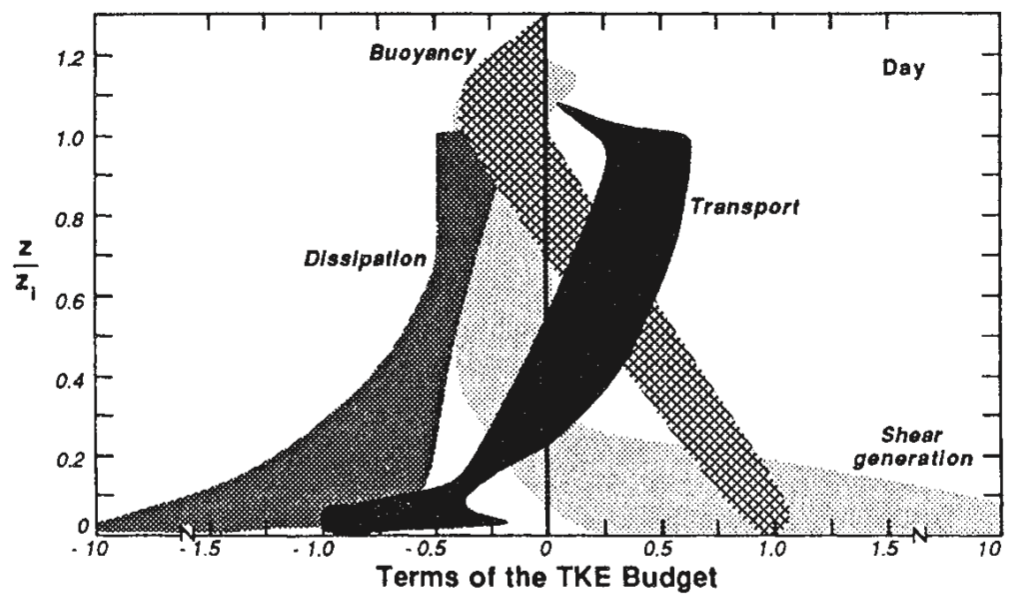
\includegraphics[width=\textwidth]{budget1}	
\end{figure}
\centering \tiny{Fig. 5.4 from Stull (1988)}
\end{frame}
%------------------------------------------------
\section{Buoyancy Variance Balance}     %
%------------------------------------------------
\framecard[colorred]{{\color{white}\Huge\begin{center}Buoyancy Variance Balance\end{center}}}
%------------------------------------------------
\begin{frame}{Buoyancy Variance Balance}
\begin{itemize}
  	\item We previously derived the following generic expression for turbulent buoyancy flux.
  	\begin{align*}
  	\frac{\partial b^\prime}{\partial t} + \frac{\partial}{\partial x_j}\left[\overline{u_j}b^\prime + u_j^\prime \overline{b} + u_j^\prime b^\prime - \overline{u_j^\prime b^\prime}\right] &= -N^2 u_j^\prime \delta_{j3} + \nu_h \frac{\partial^2 b^\prime}{\partial x_j^2}
  	\end{align*}
  	\item We will manipulate this equation to derive the buoyancy variance balance equation
  \end{itemize}
\end{frame}
%------------------------------------------------
\begin{frame}{Buoyancy Variance Balance}
\begin{itemize}
  	\item We want an expression for buoyancy variance ($\overline{b^\prime b^\prime}$).
  	\item So, we multiply by $2b^\prime$ (2 so that we can invoke the product rule)
  	\begin{align*}
  	2b^\prime\frac{\partial b^\prime}{\partial t} + 2b^\prime\frac{\partial}{\partial x_j}\left[\overline{u_j}b^\prime + u_j^\prime \overline{b} + u_j^\prime b^\prime - \overline{u_j^\prime b^\prime}\right] = &-2b^\prime N^2 u_j^\prime \delta_{j3} \\&+ 2b^\prime\nu_h \frac{\partial^2 b^\prime}{\partial x_j^2}
  	\end{align*}
  \end{itemize}
\end{frame}
%------------------------------------------------
\begin{frame}{Buoyancy Variance Balance}
\begin{itemize}
  	\item Make use of the product rule and then apply Reynolds averaging
  	\begin{align*}
  	&\frac{\partial (\overline{b^\prime b^\prime})}{\partial t} + \overline{\overline{u_j}\frac{\partial (\overline{b^\prime b^\prime})}{\partial x_j}} + 2\overline{u_j^\prime b^\prime \frac{\partial \overline{b}}{\partial x_j}} + \frac{\partial (\overline{u_j^\prime b^\prime b^\prime})}{\partial x_j} - 2\overline{b^\prime \frac{\partial \overline{u_j^\prime b^\prime}}{\partial x_j}} \\=&-2N^2 \overline{u_j^\prime b^\prime} \delta_{j3} + \nu_h \frac{\partial^2 (\overline{b^\prime b^\prime})}{\partial x_j^2} - 2\nu_h \overline{\frac{\partial b^\prime}{\partial x_j}\frac{\partial b^\prime}{\partial x_j}}
  	\end{align*}
  	\item Simplification yields
  	\begin{align*}
	\frac{\partial (\overline{b^\prime b^\prime})}{\partial t} + \overline{u_j}\frac{\partial (\overline{b^\prime b^\prime})}{\partial x_j} =&- 2\overline{u_j^\prime b^\prime} \frac{\partial \overline{b}}{\partial x_j} - \frac{\partial (\overline{u_j^\prime b^\prime b^\prime})}{\partial x_j} - -2N^2 \overline{u_j^\prime b^\prime} \delta_{j3} \\&+ \nu_h \frac{\partial^2 (\overline{b^\prime b^\prime})}{\partial x_j^2} - 2\nu_h \overline{\frac{\partial b^\prime}{\partial x_j}\frac{\partial b^\prime}{\partial x_j}}
  	\end{align*}
  \end{itemize}
\end{frame}
%------------------------------------------------
\begin{frame}{Buoyancy Variance Balance}
\begin{itemize}
  	\item Grouping terms and simplifying yields
  	\begin{empheq}[box=\widefbox]{align}
  	\label{eq2}
\underbrace{\vphantom{\overline u_j \frac{\partial (\overline{b^\prime b^\prime})}{\partial x_j}}\frac{\partial (\overline{b^\prime b^\prime})}{\partial t}}_{1} &= - \underbrace{\overline u_j \frac{\partial (\overline{b^\prime b^\prime})}{\partial x_j}}_{2} - \underbrace{2\overline{u_j^\prime b^\prime}\left[\frac{\partial \overline b}{\partial x_j} + N^2\delta_{j3} \right]}_{3}  \\&\hphantom{=\ }- \underbrace{\frac{\partial (\overline{u_j^\prime b^\prime b^\prime})}{\partial x_j}}_{4} + \underbrace{\nu_h \frac{\partial^2 (\overline{b^\prime b^\prime})}{\partial x_j^2}}_{5} -\underbrace{2\nu_h\overline{\frac{\partial b^\prime}{\partial x_j}\frac{\partial b^\prime}{\partial x_j}}}_{6}\nonumber
\end{empheq}
  \end{itemize}
\end{frame}
%------------------------------------------------
\begin{frame}{Buoyancy Variance Balance}
\textbf{\underline{Terms in Eq.~(\ref{eq2})}}
\begin{enumerate}
	\item Storage of buoyancy variance
	\item Advection of buoyancy variance by the mean wind
	\item Production of buoyancy variance by the mean buoyancy shear + stratification
	\item Transport of buoyancy variance by turbulence (turbulent diffusion)
	\item Molecular diffusion of buoyancy variance
	\item Viscous dissipation of buoyancy variance

\end{enumerate}
\end{frame}
%------------------------------------------------
\end{document}

